%%%%%%%%%%%%%%%%%%%%%%%%%%%%%%%%%%%%%%%%%%%%%%%%%%%%%%%%%%%%%%%%%%%%%%
\NeedsTeXFormat{LaTeX2e}
\documentclass[12pt,a4paper]{article}

%-- used packages ------------------------------------------------------

\usepackage{amsmath}
\usepackage{amssymb}
\usepackage{epsfig}
\usepackage{graphicx}
\usepackage{cite}
%\usepackage{mcite}
%-- page parameters -------------------------------------------------

\jot = 1.5ex
\parskip 5pt plus 1pt
\parindent 0pt
\evensidemargin -0.1in   \oddsidemargin  -0.1in
\textwidth  6.45in       \textheight 9.1in
\topmargin -1.0cm        \headsep    1.0cm

%-- command (re)definitions -----------------------------------------


\newcommand{\capdef}{}
%\newcommand{\mycaption}[2][\capdef]{\renewcommand{\capdef}{#2}%
%       \caption[#1]{{\itshape #2}}}
\newcommand{\mycaption}[2][\capdef]{\renewcommand{\capdef}{#2}%
       \caption[#1]{{\footnotesize #2}}}
\makeatletter
\renewcommand{\fnum@table}{\textbf{\tablename~\thetable}}
\renewcommand{\fnum@figure}{\textbf{\figurename~\thefigure}}
\makeatother
\def\ltap{\ \raisebox{-.4ex}{\rlap{$\sim$}} \raisebox{.4ex}{$<$}\ }
\def\gtap{\ \raisebox{-.4ex}{\rlap{$\sim$}} \raisebox{.4ex}{$>$}\ }

\newcounter{myenumi}
\newcommand{\myitem}{\refstepcounter{myenumi}\item}
\renewcommand{\themyenumi}{\roman{myenumi}}
\newenvironment{mylist}{%
        \setcounter{myenumi}{0}
        \begin{list}{\textit{\themyenumi)}}{%
        \setlength{\topsep}{0.2\baselineskip}%
        \setlength{\partopsep}{-\topsep}%
        \setlength{\itemsep}{\topsep}%
        \setlength{\parsep}{0\baselineskip}%
        \setlength{\leftmargin}{0em}%
        \setlength{\listparindent}{\parindent}%
        \setlength{\itemindent}{2.5em}%
        \setlength{\labelwidth}{1.5em}%
        \setlength{\labelsep}{0.75em}}}%
{\end{list}}

\newlength{\myem}
\settowidth{\myem}{m}
\newcommand{\sep}[1]{#1}
\newcounter{mysubequation}[equation]
\renewcommand{\themysubequation}{\alph{mysubequation}}
\newcommand{\mytag}{\stepcounter{mysubequation}%
\tag{\theequation\protect\sep{\themysubequation}}}
\newcommand{\globallabel}[1]{\refstepcounter{equation}\label{#1}}

\makeatletter
\renewcommand{\section}{\@startsection{section}{1}{0em}{-\baselineskip}%
{\baselineskip}{\normalfont\large\bfseries}}
\renewcommand{\subsection}%
{\@startsection{subsection}{2}{0em}{-0.7\baselineskip}%
{0.7\baselineskip}{\normalfont\bfseries}}
\makeatother

\newcommand{\ie}{{\it i.e.}}
\newcommand{\Ie}{{\it I.e.}}
\newcommand{\eg}{{\it e.g.}}
\newcommand{\Eg}{{\it E.g.}}
\newcommand{\cf}{{\it cf.}}
\newcommand{\etc}{{\it etc.}}
\newcommand{\eq}{Eq.}
\newcommand{\eqs}{Eqs.}
\newcommand{\Def}{Definition}
\newcommand{\fig}{Fig.}
\newcommand{\Fig}{Fig.}
\newcommand{\figs}{Figs.}
\newcommand{\Figs}{Figs.}
\newcommand{\Ref}{Ref.}
\newcommand{\Refs}{Refs.}
\newcommand{\Sec}{Sec.}
\newcommand{\Secs}{Secs.}
\newcommand{\Chapt}{Chapter}
\newcommand{\Chapts}{Chapters}
\newcommand{\Part}{Part}
\newcommand{\App}{Appendix}
\newcommand{\Apps}{Appendices}
\newcommand{\Tab}{Table}
\newcommand{\Tabs}{Tables}

\newcommand{\bi}{\begin{itemize}}
\newcommand{\ei}{\end{itemize}}
\newcommand{\ra}{$\rightarrow$}
\newcommand{\be}{\begin{equation}}
\newcommand{\ee}{\end{equation}}
\newcommand{\bea}{\begin{eqnarray}}
\newcommand{\eea}{\end{eqnarray}}
\newcommand{\nn}{\nonumber}
\newcommand{\ldm}{\Delta m_{31}^2}
\newcommand{\sdm}{\Delta m_{21}^2}
\newcommand{\deltacp}{\delta_{\mathrm{CP}}}
\newcommand{\stheta}{\sin^2 2 \theta_{13}}

\newcommand{\JHFSK}{{\sc JHF-SK}}
\newcommand{\NUMI }{{\sc NuMI}}
\newcommand{\ReactorI}{{\sc Reactor-I}}
\newcommand{\ReactorII}{{\sc Reactor-II}}
\newcommand{\JHFHK}{{\sc JHF-HK}}
\newcommand{\NuFactI}{{\sc NuFact-I}}
\newcommand{\NuFactII}{{\sc NuFact-II}}

\newcommand{\GLOBES}{{\sf GLoBES}}
\newcommand{\AEDL}{{\sf AEDL}}
\newcommand{\EDM}{{\sf EDM}}

\newcommand{\equ}[1]{\eq~(\ref{equ:#1})}
\newcommand{\figu}[1]{\fig~\ref{fig:#1}}
\newcommand{\tabl}[1]{\Tab~\ref{tab:#1}}
\newcommand{\tb}{\hspace*{3ex}}

\begin{document}
%%%%%%%%%%%%%%%%%%%%%%%%%%%%%%%%%%%%%%%%%%%%%%%%%%%%%%%%%%%%%%%%%%%%%
%%%%                     Title-page                              %%%%
%%%%%%%%%%%%%%%%%%%%%%%%%%%%%%%%%%%%%%%%%%%%%%%%%%%%%%%%%%%%%%%%%%%%%

\begin{titlepage}

% the footnote symbols are only redefined for the title page !
\renewcommand{\thefootnote}{\alph{footnote}}

\vspace*{-3.cm}
\begin{flushright}
TUM-HEP-5XX/04\\
MPP-2004-YY\\
%hep-ph/
\end{flushright}

\vspace*{0.5cm}

\renewcommand{\thefootnote}{\fnsymbol{footnote}}
\setcounter{footnote}{-1}

{\begin{center}
{\Large\bf Simulation of long-baseline neutrino oscillation
experiments with GLoBES}
\end{center}}
{\begin{center}
{\large\bf (General Long Baseline Experiment Simulator)}
\end{center}}
\renewcommand{\thefootnote}{\alph{footnote}}

\vspace*{.8cm}
%\vspace*{.3cm}
{\begin{center} {\large{\sc
                P.~Huber\footnote[1]{\makebox[1.cm]{Email:}
                phuber@ph.tum.de},~
                M.~Lindner\footnote[2]{\makebox[1.cm]{Email:}
                lindner@ph.tum.de},~and~
                W.~Winter\footnote[5]{\makebox[1.cm]{Email:}
                wwinter@ph.tum.de}
                }}
\end{center}}
\vspace*{0cm}
{\it
\begin{center}

\footnotemark[1]${}^,$\footnotemark[2]${}^,$\footnotemark[3]%
       Institut f\"ur theoretische Physik, Physik--Department,\\
       Technische Universit\"at M\"unchen,
       James--Franck--Strasse, D--85748 Garching, Germany


\end{center}}

\vspace*{1cm}


\begin{abstract}
This is the abstract.
\end{abstract}


\vspace*{.5cm}


\end{titlepage}




\newpage

\renewcommand{\thefootnote}{\arabic{footnote}}
\setcounter{footnote}{0}

%%%%%%%%%%%%%%%%%%%%%%%%%%%%%%%%%%%%%%%%%%%%%%%%%%%%%%%%%%%%%%%%%%%%%
%                     Introduction                                  %
%%%%%%%%%%%%%%%%%%%%%%%%%%%%%%%%%%%%%%%%%%%%%%%%%%%%%%%%%%%%%%%%%%%%%


\section{Introduction}

\begin{figure}[t]
\begin{center}
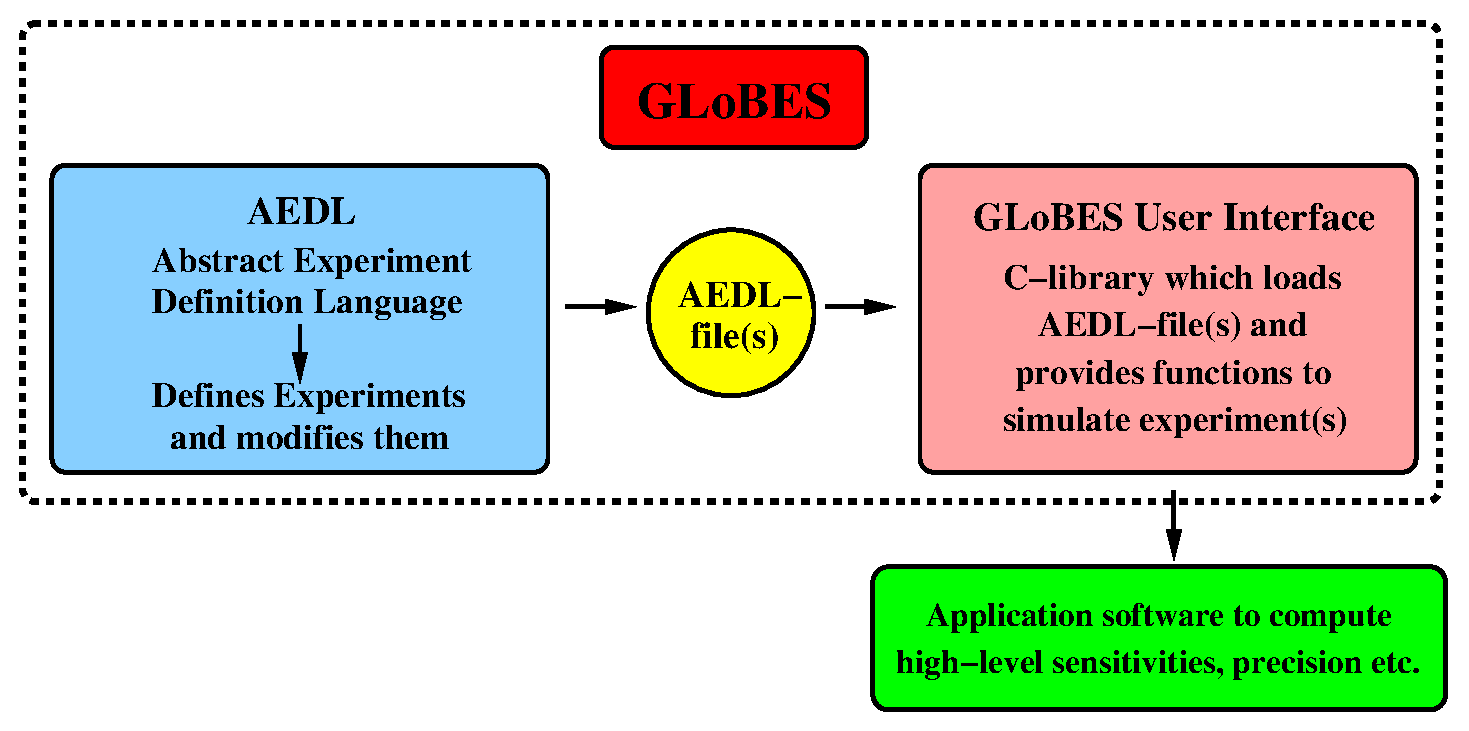
\includegraphics[width=16cm]{GLOBES}
\end{center}
\caption{\label{fig:GLOBES} General concept of the \GLOBES\ package.}
\end{figure}

\bi
 \item 
  \figu{GLOBES} and main features
 \item
  Physics basics: For what purpose? What are difficulties
 \item
  Detector simulation: What happens there?
 \item
  References for work done with \GLOBES\
 \item
  Parts of \GLOBES\
 \item 
  \figu{GLOBES} and main features
\ei

\section{The computation of raw event rates}

In this section, we sketch the computation of 
the event rates, which is on of the core parts of the \GLOBES\
software. However, because of the compecity of this issue,
we refer to the \GLOBES\ manual~\cite{Manual} for
details.  

The differential event rate for each channel is given by
\begin{eqnarray}
\label{equ:master_event}
\frac{dn_{\beta}^{\text{IT}}}{dE'}=&&N\,\int\limits_0^\infty \int\limits_0^\infty dE\,d\hat{E}\quad
\underbrace{\Phi_{\alpha} (E)}_{\mathrm{Production}} \times \nonumber\\
&&\underbrace{\frac{1}{L^2} P_{(\alpha\rightarrow\beta)}(E,L,\rho;\theta_{23},
\theta_{12},\theta_{13},
\Delta m^2_{31},\Delta m^2_{21},\deltacp)}_{\mathrm{Propagation}}
\times \nonumber \\ &&\underbrace{\sigma^{\text{IT}}_f(E)
k_f^{\text{IT}}(E-\hat{E})}_{\mathrm{Interaction}} \times \nonumber \\
&&\underbrace{ T_f(\hat{E}) V_f(\hat{E}-E')}_{\mathrm{Detection}}\,,
\end{eqnarray}
%%%%%%%%%%%%%%%%%%%%%%%%%%%%%%%%%%%
where $\alpha$ is the initial flavor of the neutrino, 
$\beta$ is the final flavor, $\Phi_{\alpha} (E)$ is the flux of the 
initial flavor at the
source, $L$ is the baseline length, $N$ is a normalization factor, and 
$\rho$ is the matter density. The energies in this formula are given as follows:
\begin{itemize}
\item
 $E$ is the incident neutrino energy, \ie, the actual energy of the 
incoming neutrino (which is not directly accessible to the experiment)
\item
 $\hat{E}$ is the energy of the secondary particle
\item
 $E'$ is the reconstructed neutrino energy, \ie, the measured
neutrino energy as obtained from the experiment
\end{itemize}
The interaction term is composed of 
two factors, which are the total cross section 
$\sigma^{\text{IT}}_\beta(E)$ for the flavor $f$ and
the interaction type IT, and the energy distribution of the 
secondary particle $k_\beta^{\text{IT}}(E-\hat{E})$.
The detector properties are 
modeled by the threshold function $T_\beta(\hat{E})$, coming from the the 
limited resolution or the cuts in the analysis, and the energy resolution 
function $V_\beta(\hat{E}-E')$ of the secondary particle. 

Since it is a lot of effort to solve this double integral numerically,
we split up the two integrations. First, we evaluate the integral over
$\hat{E}$, where the only terms containing $\hat{E}$ are
$k_\beta^{\text{IT}}(E-\hat{E})$,  $ T_\beta(\hat{E})$, and 
$ V_\beta(\hat{E}-E')$. We define:
\begin{eqnarray}
\label{equ:e_res} 
R_\beta^{\text{IT}}(E,E')\,\epsilon_\beta^{\text{IT}}(E')
 \equiv
\int\limits_0^\infty d\hat{E} \quad T_\beta(\hat{E})\,k_\beta^{\text{IT}}(E-\hat{E})
\,V_\beta(\hat{E}-E')\,. 
\end{eqnarray}
Thus, $R_\beta^{\text{IT}}(E,E')$ describes the energy response of 
the detector, \ie , a neutrino with a (true) energy $E$ is reconstructed
with an energy between $E'$ and $E'+dE'$ with a probability
$R_\beta^{\text{IT}}(E,E') dE'$. The function $R(E,E')$ is also often called ``energy resolution function''. Actually, its internal representation
in the software is a smearing matrix. The function $\epsilon_\beta^{\text{IT}}(E')$ will be refered to as ``post-smearing efficiencies'', since it will allow us to define cuts and threshold functions {\em after} the smearing is performed, \ie, as function of $E'$. 
In addition, \GLOBES\ uses ``pre-smearing efficiencies'', which are 
evaluated {\em before} the smearing is performed, \ie, as function of $E$.
Similarly, constant event rates can be added to the event rates before or after the energy smearing, which are refered to as ``pre-smearing backgrounds'' and ``post-smearing beackground''. These types of 
efficiencies an backgrounds allow a very accurate modeling of
many factors, such as geoneutrino backgrounds, energy cuts, or
energy threshold functions.

Eventually, we can write down the number of events per bin $i$ \index{Bin} and channel $c$ as
\begin{equation}
\label{equ:channel}
n_i^c=\int_{E_i-\Delta E_i/2}^{E_i+\Delta E_i/2} dE' \quad
\frac{dn_{\beta}^{\text{IT}}}{dE'} (E') \,
\end{equation}
where $\Delta E_i$ is the bin size of the $i$th energy bin.
This means that one has to solve the integral
\begin{eqnarray}
\label{equ:events_bin}
n_i^c=N/L^2\,\int_{E_i-\Delta E_i/2}^{E_i+\Delta E_i/2} dE' 
\quad \int\limits_0^\infty dE \,\, \Phi^c(E)\,
P^c(E)\,
\sigma^c(E)\,
R^c(E,E')\,
\epsilon^c(E')\,,
\end{eqnarray} 
which gives the raw event rates of the channel $c$ in the $i$th bin.
Note that the events are binned according to their \emph{reconstructed} energy.

Core part of the event rate computation is the energy smearing algorithm
to evaluate \equ{events_bin}, where either a particular energy resolution
 function can be chosen for automated energy smearing, or the discretized
smearing matrix $R^c(E,E') = R^c_{ij} $ can be given manually. In addition, it is possible
to define a low-pass filter to avoid aliasing effects for neutrino
oscillations faster that the sampling width.

\section{Definition of experiments with \AEDL\ (Abstract Experiment 
Defintion Language)}

\begin{figure}[t]
\begin{center}
\begin{tabular}{p{5cm}p{5cm}p{5cm}}
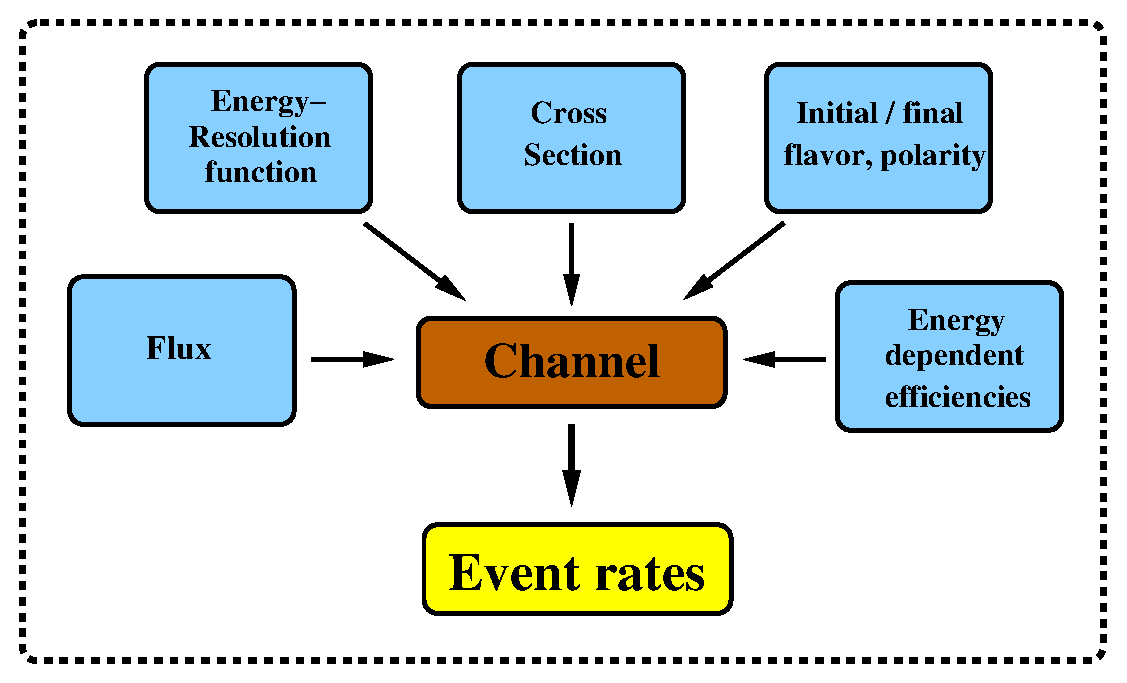
\includegraphics[width=5cm]{AEDL1} &
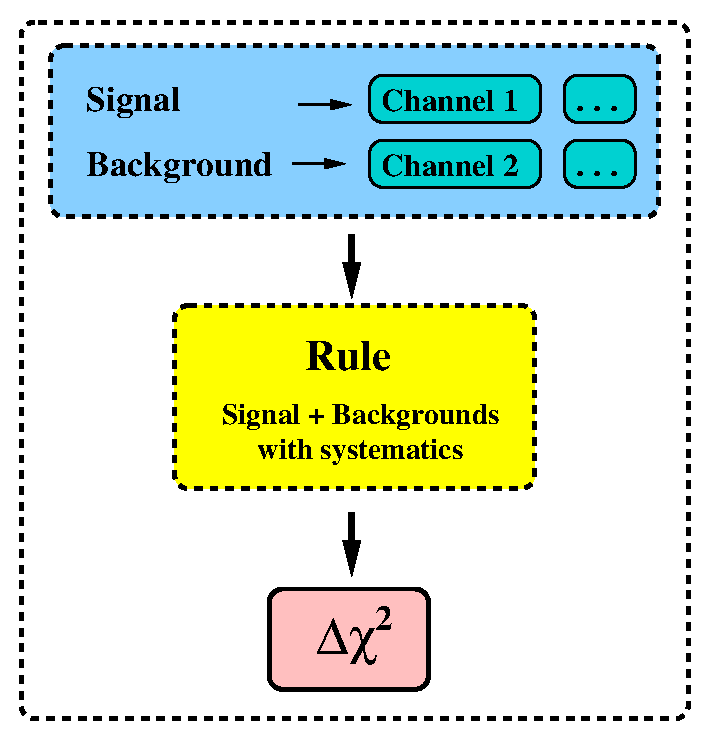
\includegraphics[width=5cm]{SignalBackground} &
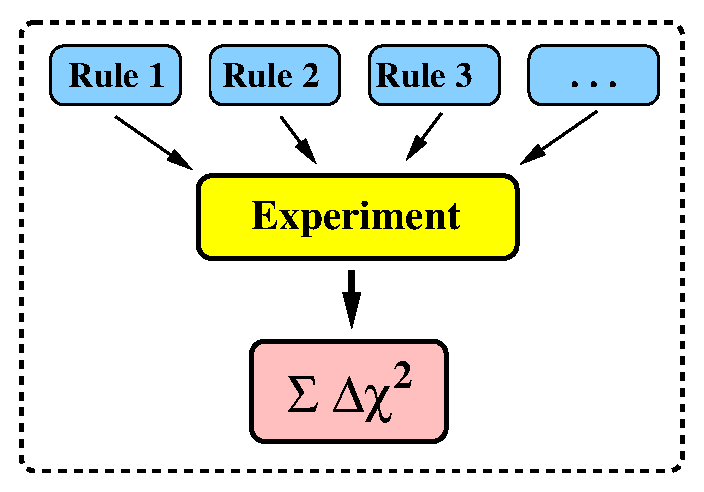
\includegraphics[width=5cm]{Rules} \\
\end{tabular}
\end{center}
\caption{\label{fig:aedl} The most important components of \AEDL :
Channels, rules, and experiments.}
\end{figure}

In order to define experiments, \GLOBES\ uses \AEDL\ (``Abstract
Experiment Definition Language''). An experiment normally corresponds
to an \AEDL\ file, which is a text file written in \AEDL\ syntax.

The main parts of any \AEDL\ experiment definition are channels,
rules, and experiments (\cf, \figu{aedl}). A channel corresponds to a neutrino oscillation channel including flux, cross section (for one specific interaction type), energy resolution function, initial and final neutrino flavors, their polarity (neutrinos or antineutrinos), and efficiencies. The channel raw event rates are computated according to \equ{events_bin}. Each channel leads to the raw event rates for a 
specfifc interaction type. In \AEDL , many of the channel components
have to be defined or loaded from files before, such as fluxes, 
cross sections, or the energy resolution function. For the
different options, see the \GLOBES\ manual~\cite{Manual}.

For a ``rule'', the raw event rates of one or more signal channels and
one or more background channels are added. The splitting in signal and
background is arbitrary, but all of the signal and background components
are defined to have a common systematics. The event rates of all 
signal and background components add up to the total event rate of the
rule, which leads to a $(\Delta \chi^2)_r$. The signal or background
within each rule allows the specification of signal and background normalization errors and energy tilt or calibration errors. 
These systematical errors will be evaluated with the ``pull method''
with the help of nuisance parameters REFERENCE. In addition to these
systematics errors, an overall evaluation strategy is assigned 
to each rule, which specifies the type of systematics (tilt or calibration
error), and the use of spectral information or total event rates.   

Finally, one ore more rules add up to an experiment, where the
total $\Delta \chi^2$ is obtained as the sum of the $\Delta \chi^2$
of all rules. This approach allows the definition of 
appearance and disappearance channels, neutrino and antineutrino running, or interaction types with different systematics (spectral information
versus counting rate) within one experiment. The \GLOBES\ user interface
allows the simulation of one or more experiment simultaneously, which
means that one could also use different experiments for different
oscillation channels. However, there is still one component missing
in the experiment definition, which is the matter density profile.
For an experiment, an arbitrary matter density profiles can be specified, which is evaluated with the evolution operator method REFERENCES.
In addition, the matter density profile is multiplied by the matter
density scaling factor, which is treated as an independent parameter
with a relative (matter density) uncertainty. With this
approach, one can take into account that the matter density profile along a specific baseline is only known to about $3\%-5\%$. Therefore, it makes
sense to combine the rules of one baseline in one experiment,
since for all of these rules the matter density profile is equal.

\section{Simulation of experiments: The C user's interface}

Minimizers?

\section{Complexity and computational issues}

\bi
\item
 Complexity of projection: $\mathcal{O}(n^7)$ (incl. matter density) API
 $\rightarrow$ Polynomical, but large effort;
 Approach with Local minimizer \ra\ $\mathcal{O}(1000)$ steps
\item
 Running time of detector simulation: (each step above)
 bins times sampling points + sampling points times matter profile steps.
 Normally dominated by first summand; for many matter profile steps
 second dominates
\item
 Computational effort: Estimates (time)
\item
 Pre-computation of smearing matrices, Spezielles
 Format bei dem Nullen nicht mitgerechnet;
  oscillation probabilities nur einmal gleichzeitig fuer alls
  Oszillationskanaele und alle ENergien berechnet
\ei
 
\section{Use of program}

\bi
\item
 Whole package
\item
 Shared library, globes command, Examples, Experiment protoypes
\item
 Manual \cite{Manual}
\ei

\section{Summary and conclusions}



%%%%%%%%%%%%%%%%%%%%%%%%%%%%%%%%%%%%%%%%%%%%%%%%%%%%%%%%%%%%%%%%%%%%%%
%%%%%%%%%%             References                         %%%%%%%%%%%%
%%%%%%%%%%%%%%%%%%%%%%%%%%%%%%%%%%%%%%%%%%%%%%%%%%%%%%%%%%%%%%%%%%%%%% 

\newpage
\bibliographystyle{./apsrev}
\bibliography{./references}

\end{document}

